
\section{Implementation}
\label{sec:impl}

We now describe the implementation of the \ix prototype. We start with
an overview of the system itself, including the separation of control
plane and dataplane, the use of virtualization hardware for
protection, and resource allocation (\S\ref{sec:impl:overview}). We
then describe salient aspects of our system, including the internals
of the \ix kernel and in particular its pipeline
(\S\ref{sec:impl:kernel}), the native API at the kernel/user boundary
(\S\ref{sec:impl:api}), our approach to compatibility
(\S\ref{sec:impl:libix}), and finally our approach to flow control and
congestion management (\S\ref{sec:impl:net}).  We close with a
discussion of our approach, its current implementation restrictions,
and directions for future work (\S\ref{sec:impl:discussion}).

\subsection{System Architecture}
\label{sec:impl:overview}

\begin{figure}
\begin{centering}
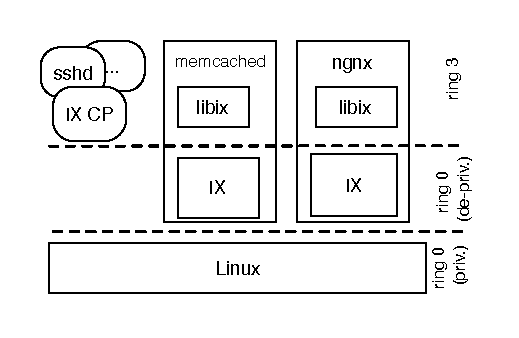
\includegraphics{figs/cp-dp.eps}
\centering\caption{Protection and separation in \ix.}
\label{fig:cp-dp}
\end{centering}
\end{figure}



The system architecture of \ix addresses the design goals of providing
separation and protection to both control and dataplane, and to
provide an elastic allocation of resources.  Our first implementation
decision was to operate the control plane as part of a standard Linux
environment.  This choice is driven by a dual observation. First,
Linux is already the operating system of choice for most web-scale
datacenters; by using Linux as its control plane foundation, \ix
immediately benefits from the broad hardware compatibility and deep
integration into systems management framework offered by Linux
distributions. Second, Linux provides the necessary resource
allocation mechanisms to provide coarse-grain, elastic allocation of
resources.  The control plane relies on these mechanisms to
provision and control the dataplane.  For example, core allocation can
be precisely controlled through real-time priorities and
\texttt{cpumasks}; memory can be allocated in 2MB and 1GB chunks from
specified NUMA nodes; PCI devices and virtual functions alike can be
assigned to specified processes, etc.

Our second implementation decision was to build the \ix dataplane on
top of the Dune~\cite{belay2012dune} framework.  Dune is a Linux
kernel module and library that uses the ubiquitous VT-x
virtualization hardware~\cite{DBLP:journals/computer/UhligNRSMABKLS05}
found in current Intel processors to run untrusted processes in kernel
model.  These processes in turn can safely use virtualized hardware
resources such as page tables to run untrusted applications.

Fig.~\ref{fig:cp-dp} illustrates our implementation choices.  The \ix
control plane is a combination of Linux scripts and daemons that
launch, monitor and control the \ix dataplanes. The dataplane consists
of the \ix kernel, which directly operates on the NIC hardware queues
and runs the network protocol processing stack, and then launches and
runs a single, event-driven application at userlevel.

\subsection{Global Resource Management}

The implementation separates global resource mechanisms from policies
as follows: the mechanisms are implemented by an enhanced version of
Dune and are independent of the choice of the dataplane kernel.  The
policies however rely on the cooperation between the control plane and
dataplane kernels.

\myparagraph{Mechanisms:}
This architecture is explicitly designed to favor scalability and
performance at the possible expense of fine-grain resource management.
This is true for CPU, memory, and network I/O resources, which are
allocated exclusively to a dataplane until explicitly revoked.  The
unit of CPU resource allocation is the hyperthread.  Hyperthreads are
allocated to a dataplane until they are explictly revoked, using a
protocol similar to the one used in
Exokernels~\cite{DBLP:conf/sosp/EnglerKO95}.  In this approach,
although the Linux kernel is \emph{in fine} in control of the
machine, the system minimizes any run-time interference.  The use of
\texttt{cpumasks} for processes and I/O device interrupts alike,
ensures that the dataplane can operate with negligible unsolicited
interference from the controlling OS.

Memory is allocated at coarse granularity as a combination of 2MB and
1GB pages and protected using Extended Page Tables.  The use of
superpages reduces the overheads of two-dimensional page
walking~\cite{DBLP:conf/asplos/BhargavaSSM08}.  Memory revocation is
not supported in the design, and neither is any form of system-level
paging.  Instead, each dataplane is launched with a specific memory
allocation that is guaranteed to be resident.

Finally, network I/O devices and in particular descriptor rings are
also allocated exclusively to a dataplane using an approach based on
\edb{VFIO?}~\cite{missing}, similar to the one used by userlevel
networking stacks.

\myparagraph{Policies:}
In contrast to the mechanisms, which are generic, different policies
can be envisioned to meet different use cases and optimization
functions.  If neither energy proportionality or server consolidation
is of any concern, the control plane can obviously launch a single
dataplane instance configured with the maximal available physical
resources.  In more realistic scenarios, the dataplane is
``right-sized'' to meet its service-level agreements with minimal
resource allocations.  The control plane can further dynamically add
or revoke CPUs from a dataplane instances, e.g., when the dataplane
signals some sustained congestion or violation of its service-level
agreements, or conversely when the allocated CPU resources are
underutilized.

%\begin{figure}
\begin{centering}
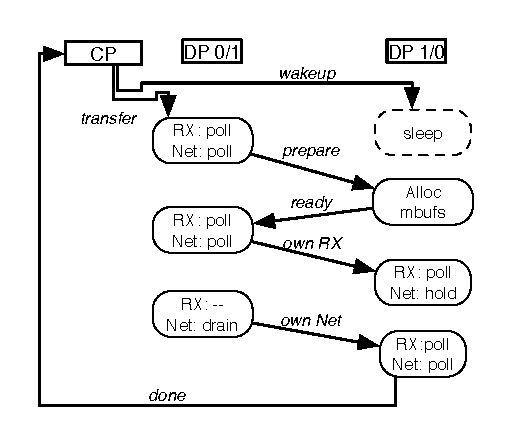
\includegraphics{figs/queue-takeover.eps}
\caption{Queue takeover algorithm.}
\label{fig:queue-takeover}
\end{centering}
\end{figure}



\subsection{The \ix Kernel}
\label{sec:impl:kernel}

The \ix kernel merges two distinct functions, as it is both an
operating system and a dataplane.

\begin{figure}
\hspace*{-0.25in}\centering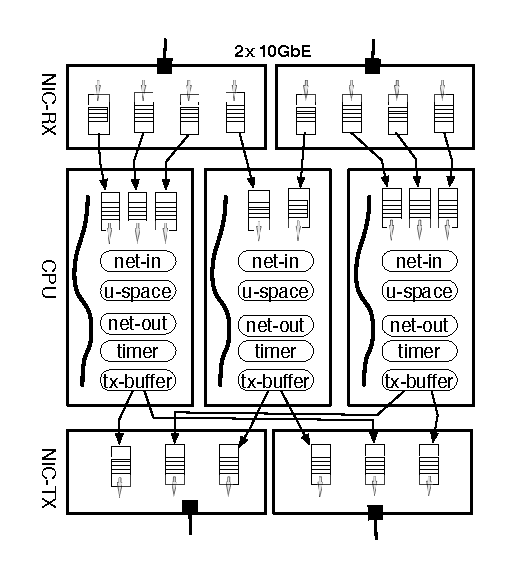
\includegraphics{figs/queues-cores.eps}
\caption{Example of IX scaling across two NICs interfaces, 8 NIC RX queues, and 3 CPU hardware threads.} 
\label{fig:queues-cores}
\end{figure}



First, \ix is an single address-space OS that can launch and run
legacy, multi-threaded POSIX applications.  We use the sandboxing
mechanisms of Dune to load the application and its libraries in the
address space, and then intercept and if necessary redirect system
calls to the underlying Linux operating system. We extend these
mechanisms, and in particular \texttt{pthreads}, to create two
categories of threads: elastic threads, which can initiate and consume
network I/O with the dataplane, and background threads, which perform
auxiliary functions.  Only the elastic threads are part of the
dataplane: at initialization time, the application pre-allocates one
elastic thread for each of the configured maximum CPU for the
dataplane; at run-time, these threads are either enabled, in which
case they continuously run through the \ix pipeline, or blocked
revocation by the control plane.  Elastic threads are not expected to
perform blocking POSIX system calls as this would prevent the further
processing of network events.  In contrast, background threads operate
like any vanilla pthreads and share the application's address space,
and can routinely block on I/O.

Second, \ix is a dataplane that expose safely the TCP/IP family of
protocols directly to the elastic threads without going through the
familiar socket abstraction and API layer.  Each elastic thread
manages a non-overlapping set of hardware queues to receive and send
packets directly to the Ethernet NIC hardware.
Fig.~\ref{fig:queues-cores} illustrates the various stages of the \ix
dataplane: (i) it polls the receive queues of the NIC to dequeue all
newly received packets into an in-memory queue, and post fresh
descriptors; (ii) process a bounded number of packets through the
incoming networking stack, with the side-effect of generating an
array of events; (iii) passes control to the user-space applications,
which processes all outstanding events, with the application
responding by generating an array of \ix commands.  (iv) upon return
of control from user-space, \ix processes all outstanding commands,
including the ones that direct outgoing networking traffic; (v) run
all kernel timers, in particular to ensure compliant TCP behavior;
(vi) enqueue the all outgoing Ethernet frames into the hardware
descriptor ring.


\subsection{The \ix native API}
\label{sec:impl:api}

\begin{figure}
\begin{centering}
% FIXME
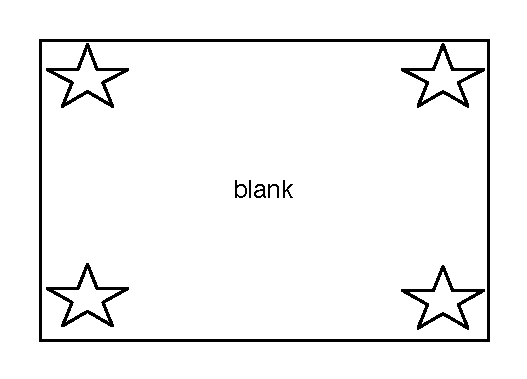
\includegraphics{figs/blank.eps}
\caption{Zero-copy, event-driven ping-pong server using the native \ix API.}
\label{fig:listing}
\end{centering}
\end{figure}



\todo Fig.~\ref{fig:listing} \christos{if we can sqeeze in an app example (pseudocode for echo
  server) it would be great}


\todo list of events (is it like Megapipe and/or mTCP)

\todo  true zero-copy

\todo discuss shared mbufs (read-only mappings)

\subsection{Protocol Stack and Device Driver}

The \ix kernel includes a complete network protocol stack with
RFC-compliant support for TCP, UDP, ARP, ICMP and LACP.  It however
explicitly lacks a complete IP-layer and is therefore only a capable
networking endpoint, but not of handling routing, bridging or
filtering functions.  It also totally lacks a socket layer and its
associated API and semantics.  For our implementation of TCP, we chose
to LWIP~\cite{} as a starting point for our code base because of its
modularity and is maturity as a compliant, feature-rich networking
stack.  LWIP was however designed with memory-efficiency in mind,
primarily for embedded environments.  We radically changed the data
structures that organize protocol control blocks for scalability, as
well as for finer-grain, precise timer management.  However, we did
not (yet) attempt to optimize the code paths for performance, and
consequently believe that our results have room for improvement.

The \ix kernel supports a modular device driver interface, with an
original focus on the Intel XXX device.  We used
DPDK~\cite{intel:dpdk} as a starting code base, but substantially
rewrote it for performance, in particular in the area of
\adam{fill-in}.  The driver supports directly accesses hardware
queues, which are mapped into memory by the Dune framework and
supports all major hardware offloads.  It supports multi-queue
configurations with RSS up to the hardware limit (16) and multiple NIC
within the same dataplane.  Because of restrictions in the use of VT-d
in particular in the area of \adam{XXXX}, the device operates without
an IOMMU.  Instead, the driver directly populates descriptors with
host-physical addresses, which are provided by by Dune framework as a
form of paravirtualization~\cite{DBLP:conf/sosp/BarhamDFHHHN03}.



\subsection{Congestion management and flow control}
\label{sec:impl:net}

Unlike a traditional in-kernel stack, which decouples protocol
processing from the applications, \ix keeps them strongly coupled and
avoids introducing new abstractions.  As a result, congestion
management and flow control are more directly made visible to the
applications.

First, the \ix dataplane centralizes all congestion management
mechanisms and policies at the NIC edge of the system, i.e., before
the packets are processed by the other stages of the pipeline, so that
no other part of the system may necessarily allocate or buffer the
packet.  Unlike a traditional implementation of POSIX sockets, where
the protocol layer may buffer out-of-order packets, the upper layer
can temporarily refuse packets, and the packets are ultimately copied
into userspace, \ix always delivers streams to applications without
copying in a read-only portion of the address space, and drops
out-of-order packets.

The implementation mechanism for congestion management is trivial - we
start by moving all incoming packets from the hardware ring into a
corresponding in-memory queue, but only process a bounded batch of
packets at each iteration.  The pipeline then processes the buffer up
to the point where it is either dropped or passed to userspace.  This
has a number of benefits.  First, we make use of extensive DRAM
resources to handle bursty congestion that can occur on an 10GbE
fabric, if the application is under-provisioned in terms of CPU
resources, or is going through an atypically expensive operation such
as garbage collection.  Second, the resulting in-memory queue can
serve as the basis for extensive monitoring of service-level agreement
expressed in terms of queuing delays.  Third, it provides a convenient
location to implement congestion management policies such as
ECN~\cite{ramakrishnan2001addition} or
RED~\cite{DBLP:journals/ton/FloydJ93}.

The system would however not be stable without also ensuring flow
control.  Acknowledgments are sent by the networking stack only when
packets are processed by the dataplane.  Congestion in the NIC edge
therefore leads to shrinking windows in peers.  In contrast, traditional stacks
acknowledge packets well before they are processed by application and
buffer in the socket layer.

When sending, flow control is safely, but directly exposed to
user-space applications.  To each send call, the \ix kernel generate a
corresponding event with the number of bytes actually sent, and a
second corresponding event to the numbers of bytes acknowledged by
the peer.  These two events together provide a direct view of the
sliding window to application and provide the foundation for zero-copy,
non-blocking operations.  In contrast here also, traditional stacks
buffer and copy on the send side.


\subsection{LibEvent Compatibility}
\label{sec:impl:libix}
\todo Details 

\subsection{Discussion}
\label{sec:impl:discussion}

Although only a prototype, \ix is capable of running complete,
real-world applications.  We learned a number of lessons during the
course of its implementation.

\todo challenges in API design

\todo any loose ends

\todo explicitly list future work (more complete TCP, policies for elasticity)

\todo polling vs. interrupts

\todo run-time elasticity

\todo benefits of explicit congestion maangemetn adn flow control ... end-to-end principle, ... 

